%%%%%%%%%%%%%%%%%%%%%%%%%%%%%%%%%%%%%%%%%%%%%%%%%%%%%%%%%%%%%%%%%%%%%%%%%%%%%%%%
% Poster Template (Oxford/I6pd2 Lineage)
% Original:
%   A beamer poster style for the University of Oxford
%   Atilim Gunes Baydin <gunes@robots.ox.ac.uk>, Nov 2016
%   Based on the I6pd2 style by Thomas Deselaers and Philippe Dreuw
%
% Upstream reference:
%   Dreuw & Deselaers' LaTeX Beamer Poster Template (v1.0, 2013-11-04)
%   http://www-i6.informatik.rwth-aachen.de/~dreuw/latexbeamerposter.php
%   Downloaded via LaTeXTemplates.com
%
% License (must retain per CC BY-NC-SA 3.0):
%   https://creativecommons.org/licenses/by-nc-sa/3.0/
%   You must keep attribution; noncommercial use; share alike.
%
% Local note:
%   Modified for Rice University poster template.
%   Maximum size: 48" × 36" (landscape).
%%%%%%%%%%%%%%%%%%%%%%%%%%%%%%%%%%%%%%%%%%%%%%%%%%%%%%%%%%%%%%%%%%%%%%%%%%%%%%%%

%------------------------------------------------------------------------------
% Document class and poster canvas
%------------------------------------------------------------------------------
\PassOptionsToPackage{pdfpagelabels=false}{hyperref}
\documentclass[final,14pt]{beamer}

% Exact poster layout (48in x 36in, landscape). Scale controls internal font/layout scaling.
% Fits within Energy HPC & AI Conference max 48" × 48" requirement.
\usepackage[orientation=landscape,width=48in,height=36in,scale=1.45]{beamerposter}

% Explicit paper size (often redundant with beamerposter, but retained from source)
\geometry{paperwidth=48in,paperheight=36in}

%------------------------------------------------------------------------------
% Debug helpers
%------------------------------------------------------------------------------
% \showfontsize -> prints current font size (pt)
\makeatletter
\newcommand{\showfontsize}{\f@size{} pt}
\makeatother

%------------------------------------------------------------------------------
% Theme selection
%------------------------------------------------------------------------------
\usetheme[poster]{Rice}

%------------------------------------------------------------------------------
% Encodings, fonts, basic utilities
%------------------------------------------------------------------------------
\usepackage[utf8]{inputenc}         % UTF-8 input
\usepackage{blindtext}              % Dummy text (for testing/layout)

% Math & theorem packages
\usepackage{amsmath,amsthm,amssymb,latexsym}

% Paragraph alignment utilities
% \usepackage[document]{ragged2e}

% Font stacks (Times/PS). professionalfonts uses installed fonts as-is.
\usepackage{times}\usefonttheme{professionalfonts}
\usefonttheme[onlymath]{serif}
% \boldmath                          % Uncomment to bold all math (usually off)

% Lists and tables
\usepackage{enumitem}
\usepackage{booktabs}                % High-quality table rules

% Micro-typography (commented in source; retained as-is)
% \usepackage{microtype}

% Additional font/PS helpers and bold math
\usepackage{pslatex,bm}

% Graphics and drawing
\usepackage{tikz}
\usepackage{caption}

% Algorithms (two common styles, both retained)
\usepackage[vlined]{algorithm2e}
\usepackage{algorithmic}
\renewcommand{\algorithmicrequire}{\textbf{Input:}}
\renewcommand{\algorithmicensure}{\textbf{Output:}}

%------------------------------------------------------------------------------
% Layout tweaks and caption template
%------------------------------------------------------------------------------
% Reduce extra space below displayed equations at \normalsize
\makeatletter
\g@addto@macro\normalsize{%
    \setlength\belowdisplayskip{-0pt}%
}
\makeatother

% Custom caption template for beamer figures (as in source)
\usecaptiontemplate{\small\structure{\insertcaptionname~\insertcaptionnumber: }\insertcaption}

%------------------------------------------------------------------------------
% Color shortcuts and minor utilities
%------------------------------------------------------------------------------
\newcommand{\shrink}{-42pt}                       % Vertical shrink amount used in content
% Color convenience macros (colors themselves defined via theme elsewhere)
% \newcommand{\mypink}{\color{myyellow}}
\newcommand{\mypink}{\color{mypink}}
\newcommand{\myorange}{\color{myorange}}
% \newcommand{\myturquoise}{\color{myblue}}
\newcommand{\myturquoise}{\color{myturquoise}}

% Local custom color example
\definecolor{myGreen}{rgb}{0,0.5,0}

% Top-align image boxes
\def\imagetop#1{\vtop{\null\hbox{#1}}}

%------------------------------------------------------------------------------
% Bibliography styling (spacing and sizes)
%------------------------------------------------------------------------------
\let\oldbibliography\thebibliography
\renewcommand{\thebibliography}[1]{\oldbibliography{#1}%
  \setlength{\itemsep}{-10pt}%
}
\setbeamerfont{bibliography item}{size=\tiny}
\setbeamerfont{bibliography entry author}{size=\footnotesize}
\setbeamerfont{bibliography entry title}{size=\footnotesize}
\setbeamerfont{bibliography entry location}{size=\footnotesize}
\setbeamerfont{bibliography entry note}{size=\footnotesize}

%------------------------------------------------------------------------------
% Math operators and common symbols (add or remove as needed for your poster)
%------------------------------------------------------------------------------
\DeclareMathOperator*{\argmin}{argmin}
\DeclareMathOperator{\diag}{diag}
\DeclareMathOperator{\trace}{tr}
\newcommand{\real}{\mathbb{R}}
\newcommand{\complex}{\mathbb{C}}
\newcommand{\nat}{\mathbb{N}}
\newcommand{\integer}{\mathbb{Z}}

%------------------------------------------------------------------------------
% Title / Author / Institute (poster) — beamer \inst numbering + hyperref-safe
%------------------------------------------------------------------------------
\title{\texorpdfstring{\Huge Your Poster Title Here}
                          {Your Poster Title Here}}

\author{\texorpdfstring{\Large
  Author Name\inst{1}\;\; Co-Author Name\inst{1}}
  {Author Name (1); Co-Author Name (1)}
}

\institute{\texorpdfstring{%
  \inst{1} Department of Computational Applied Mathematics \& Operations Research, Rice University
}{Department of Computational Applied Mathematics \& Operations Research, Rice University}}

\hypersetup{
  pdftitle  = {Your Poster Title Here},
  pdfauthor = {Author Name; Co-Author Name}
}

%------------------------------------------------------------------------------
% Footer helpers (used by some themes)
%------------------------------------------------------------------------------
\newcommand{\leftfoot}{\href{https://github.com/username}{github.com/username}}
\newcommand{\centerfoot}{Conference or Event Name}
\newcommand{\rightfoot}{\href{mailto:your.email@rice.edu}{your.email@rice.edu}}
%------------------------------------------------------------------------------

\begin{document}

% extra space below every block (tweak as needed; reduced to fix overfull vbox)
\addtobeamertemplate{block end}{}{\vspace*{0ex}}

\begin{frame}[t]

\begin{columns}[t,onlytextwidth]
  % left spacer
  % \begin{column}{.015\textwidth}\end{column}
  \hspace*{\fill} % left edge space (no fixed-width spacer)

  % =========================
  % Column 1
  % =========================
  \begin{column}{.28\textwidth}
    \vspace{\shrink}
    \vspace{-.5cm}

    % Motivation
    \begin{block}{{\Large Motivation}}
      $\blacktriangleright$ Add your first motivation point here.

      $\blacktriangleright$ Add your second motivation point here.

      $\blacktriangleright$ Add your third motivation point here.

      $\blacktriangleright$ \textbf{Goal}: Add your research goal here.
    \end{block}

    \vspace{-.3cm}

    % Methods / Approach
    \begin{block}{{\Large Methods}}
      $\blacktriangleright$ \textbf{Add method name}: Add description of your approach or framework.

      $\blacktriangleright$ \textbf{Add component name}: Add key equations or formulations here.
      \[
        \text{Add equation here}
      \]

      $\blacktriangleright$ \textbf{Add another component}: Add supporting details.

      $\blacktriangleright$ \textbf{Add discretization or setup}: Add relevant equations.
      \[
        \text{Add equation here}
      \]
    \end{block}

    \vspace{-.5cm}

    % Problem Setup / Background
    \begin{block}{{\Large Problem Setup}}
      Add your problem formulation or background here. Include equations as needed:
      \[
        \text{Add problem statement or governing equations}
      \]

      $\blacktriangleright$ \textbf{Add parameter or assumption}: Add details.

      $\blacktriangleright$ \textbf{Add test cases or setup}: Add specifics.

      $\blacktriangleright$ \textbf{Add grid or discretization}: Add numerical setup.
    \end{block}

    \vspace{-.3cm}

    % Implementation / Protocol
    \begin{block}{{\Large Implementation}}
      $\blacktriangleright$ \textbf{Add loss or objective}: Add formulation.

      $\blacktriangleright$ \textbf{Add optimization details}: Add hyperparameters, training setup.

      $\blacktriangleright$ \textbf{Add implementation detail}: Add matrix form, algorithm, etc.

      $\blacktriangleright$ \textbf{Add robustness or validation}: Add details.
    \end{block}

  \end{column}

  % middle spacer
  \begin{column}{.01\textwidth}\end{column}

  % =========================
  % Column 2
  % =========================
  \begin{column}{.31\textwidth}
    \vspace{\shrink}
    \vspace{-.5cm}

    % Algorithm / Recipe
    \begin{block}{{\Large Algorithm}}
      $\blacktriangleright$ \textbf{Add algorithm name}: Add step-by-step description of your method or procedure. Include key operations and parameters.
    \end{block}

    \vspace{-.3cm}

    % Figure 1
    \begin{block}{{\Large Results}}
      \centering
      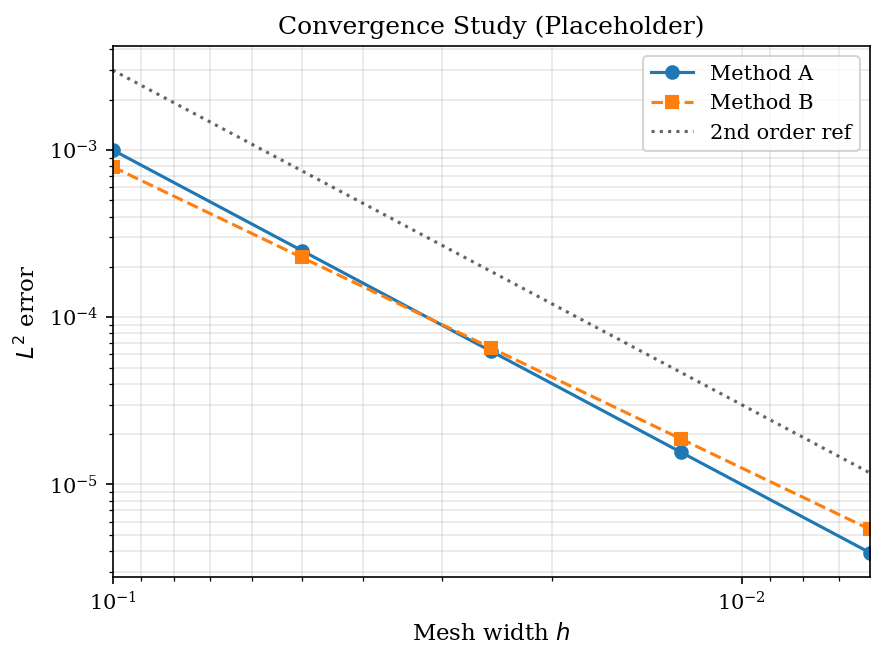
\includegraphics[width=\textwidth]{figures/content/placeholder_1.png}
      \captionof{figure}{Add figure caption here.}
    \end{block}

    \vspace{-.3cm}

    % Figure 2
    \begin{block}{{\Large Convergence}}
      \centering
      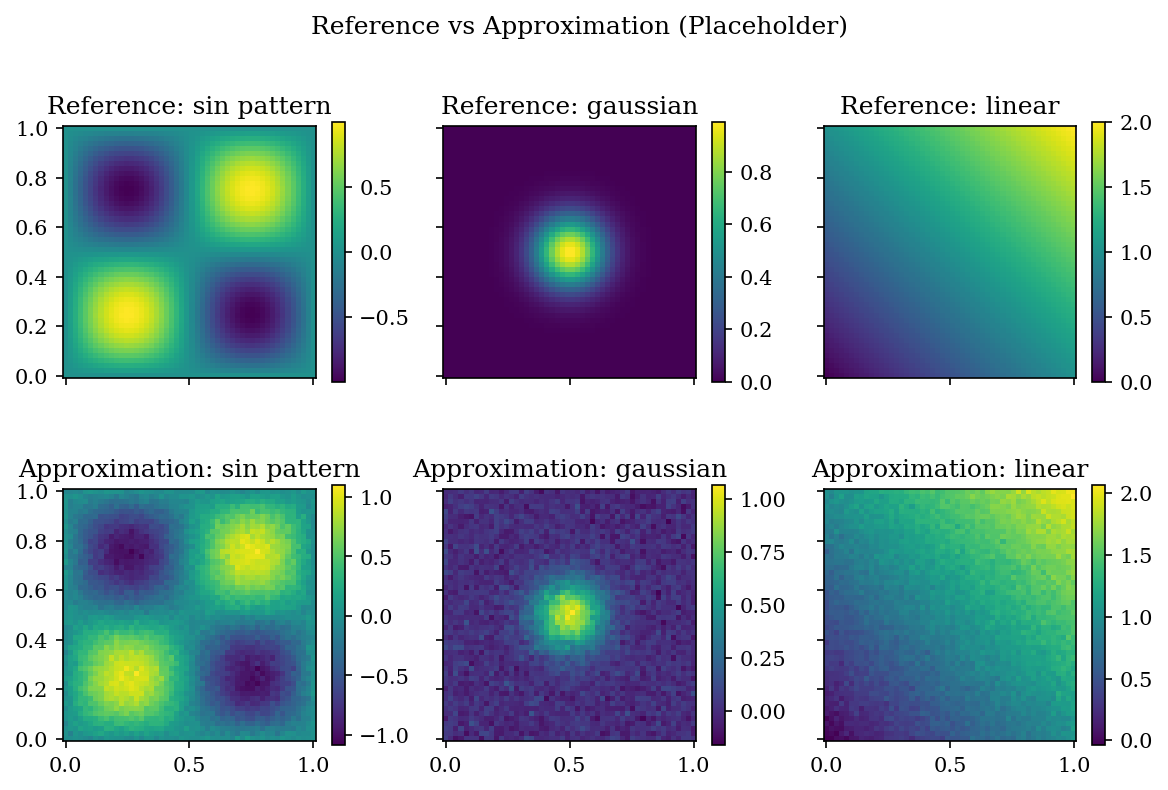
\includegraphics[width=\textwidth]{figures/content/placeholder_2.png}
      \captionof{figure}{Add figure caption here.}
    \end{block}

    \vspace{-.3cm}

    % Acknowledgments (text)
    \begin{block}{{\Large Acknowledgments}}
      \footnotesize
      Add your acknowledgments here (e.g., funding, collaborators).
    \end{block}
  \end{column}

  % middle spacer
  \begin{column}{.01\textwidth}\end{column}

  % =========================
  % Column 3
  % =========================
  \begin{column}{.38\textwidth}
    \vspace{\shrink}
    \vspace{-.5cm}

    % Key Contributions
    \begin{block}{{\Large Key Contributions}}
      $\blacktriangleright$ \textbf{Add contribution 1}: Add description of your first key contribution.

      $\blacktriangleright$ \textbf{Add contribution 2}: Add description of your second key contribution.

      $\blacktriangleright$ \textbf{Add contribution 3}: Add description of your third key contribution.
    \end{block}

    \vspace{-.3cm}

    % Figure 3 / Key Results
    \begin{block}{{\Large Key Results}}
      \centering
      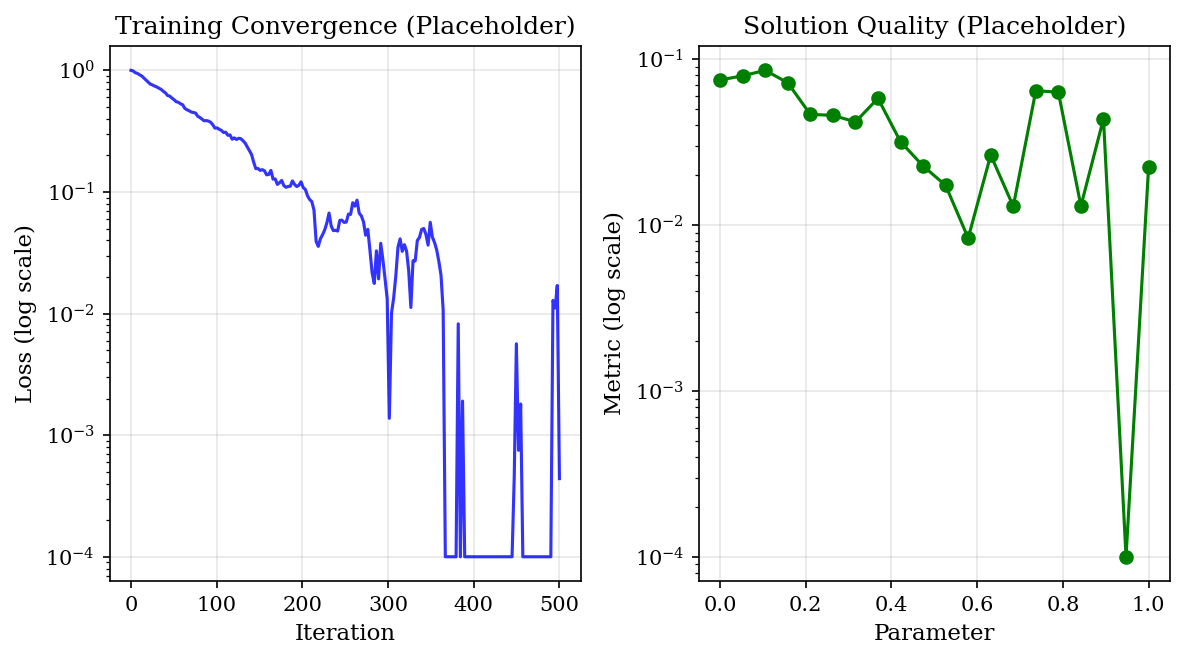
\includegraphics[width=\textwidth]{figures/content/placeholder_3.png}
      \captionof{figure}{Add figure caption here.}
      
      \vspace{0.1cm}
      
      $\blacktriangleright$ \textbf{Add finding}: Add key takeaway or validation result.
      
      $\blacktriangleright$ \textbf{Add metric or observation}: Add supporting details.
    \end{block}

    \vspace{-.3cm}

    % Conclusion
    \begin{block}{{\Large Conclusion}}
      $\blacktriangleright$ Add your first conclusion point.\\
      $\blacktriangleright$ Add your second conclusion point.\\
      $\blacktriangleright$ Add your third conclusion point (e.g., future work or impact).
    \end{block}

    % Acknowledgments (logos)
    \begin{block}{{\Large Acknowledgments}}
      \centering
      \vspace{0.2cm}
      
\includegraphics[height=2.5cm]{figures/logos/ken_kennedy_institute.png}
    \end{block}

    % Optional bibliography (kept commented intentionally)
    % \nocite{example2020book}
    % \nocite{example2021article}
    % \bibliographystyle{abbrv}
    % \bibliography{bibliography}

  \end{column}

  % right spacer
  % \begin{column}{.02\textwidth}\end{column}
  \hspace*{\fill} % left edge space (no fixed-width spacer)

\end{columns}

\end{frame}
\end{document}
